
\documentclass[11pt,a4paper]{article}
\usepackage[margin=1.1in]{geometry}
\usepackage{amsmath, amssymb, amsthm}
\usepackage{graphicx}
\usepackage{booktabs}
\usepackage{siunitx}
\usepackage{hyperref}
\usepackage{microtype}
\usepackage{physics}
\usepackage{csquotes}
\usepackage{caption}
\usepackage{listings}
\usepackage{xcolor}

\hypersetup{colorlinks=true,linkcolor=blue,citecolor=blue,urlcolor=blue}
\title{Finding a Whisper in a Storm: An Intuitive Walkthrough of LIGO-Style Matched Filtering}
\author{}
\date{\today}

\begin{document}
\maketitle

\begin{abstract}
Gravitational waves are faint ripples in spacetime, so faint that even the most sensitive instruments see mostly noise. This document tells the story of how data analysis---especially matched filtering---turns noisy strain measurements into confident detections. We build a minimal, reproducible ``toy detector'': a synthetic chirp hidden inside random noise. We then recover it using the core idea of LIGO's searches, with clear intuition about ``Gaussian'' noise and why correlation is the right question to ask of the data.
\end{abstract}

\section{Generative Model and Hypotheses}
We model the observed strain $d(t)$ as either noise alone or noise plus a signal:
\begin{align}
\mathcal{H}_0:~ d(t) &= n(t), \label{eq:h0}\\
\mathcal{H}_1:~ d(t) &= h(t) + n(t), \label{eq:h1}
\end{align}
where $n(t)$ is a (roughly) stationary random process and $h(t)$ is a deterministic template.

If the noise is (approximately) Gaussian, the likelihood ratio can be expressed with the noise-weighted inner product:
\begin{equation}
(a|b) \equiv 4\,\Re \int_{0}^{\infty} \frac{\tilde a(f)\,\tilde b^{*}(f)}{S_n(f)}\,\mathrm{d}f, \label{eq:inner}
\end{equation}
where tildes denote Fourier transforms and $S_n(f)$ is the one-sided PSD.

\section{Matched Filtering and SNR}
For a template $h$ with relative time shift $\tau$, the SNR time series is
\begin{equation}
\rho(\tau) \equiv \frac{(d | h_\tau)}{\sqrt{(h|h)}}, \qquad
h_\tau(t) \equiv h(t-\tau). \label{eq:snr}
\end{equation}
Peaks of $\rho(\tau)$ indicate times where $d$ contains $h$ most strongly, with \eqref{eq:inner} downweighting noisy bands.

\section{Whitening and Spectrograms}
To visualize features and approximate the weighting in \eqref{eq:inner}, we whiten the data:
\begin{equation}
\tilde x_{\mathrm{w}}(f) \equiv \frac{\tilde x(f)}{\sqrt{S_n(f)}}, \qquad
x_{\mathrm{w}}(t) = \mathcal{F}^{-1}\!\big[\tilde x_{\mathrm{w}}(f)\big]. \label{eq:whiten}
\end{equation}
We then compute an STFT with a long window and high overlap:
\begin{equation}
Z(t_k,f_m) \equiv \sum_{t} x_{\mathrm{w}}(t)\,w(t-t_k)\,e^{-i2\pi f_m t}, \label{eq:stft}
\end{equation}
and plot $10\log_{10}|Z|^2$ after subtracting, for each $f_m$, the median over $t_k$:
\begin{equation}
S_{\mathrm{dB}}^{\mathrm{ms}}(t_k,f_m) \equiv 10\log_{10}\!\big(|Z|^2\big)
~ - ~ \mathrm{median}_{t_k}\!\left[\,10\log_{10}\!\big(|Z|^2\big)\,\right]. \label{eq:medsub}
\end{equation}
Finally, we clip color limits to the $95$th--$99.5$th percentiles of $S_{\mathrm{dB}}^{\mathrm{ms}}$ to enhance contrast.

\section{Figures}
\begin{figure}[h!]\centering
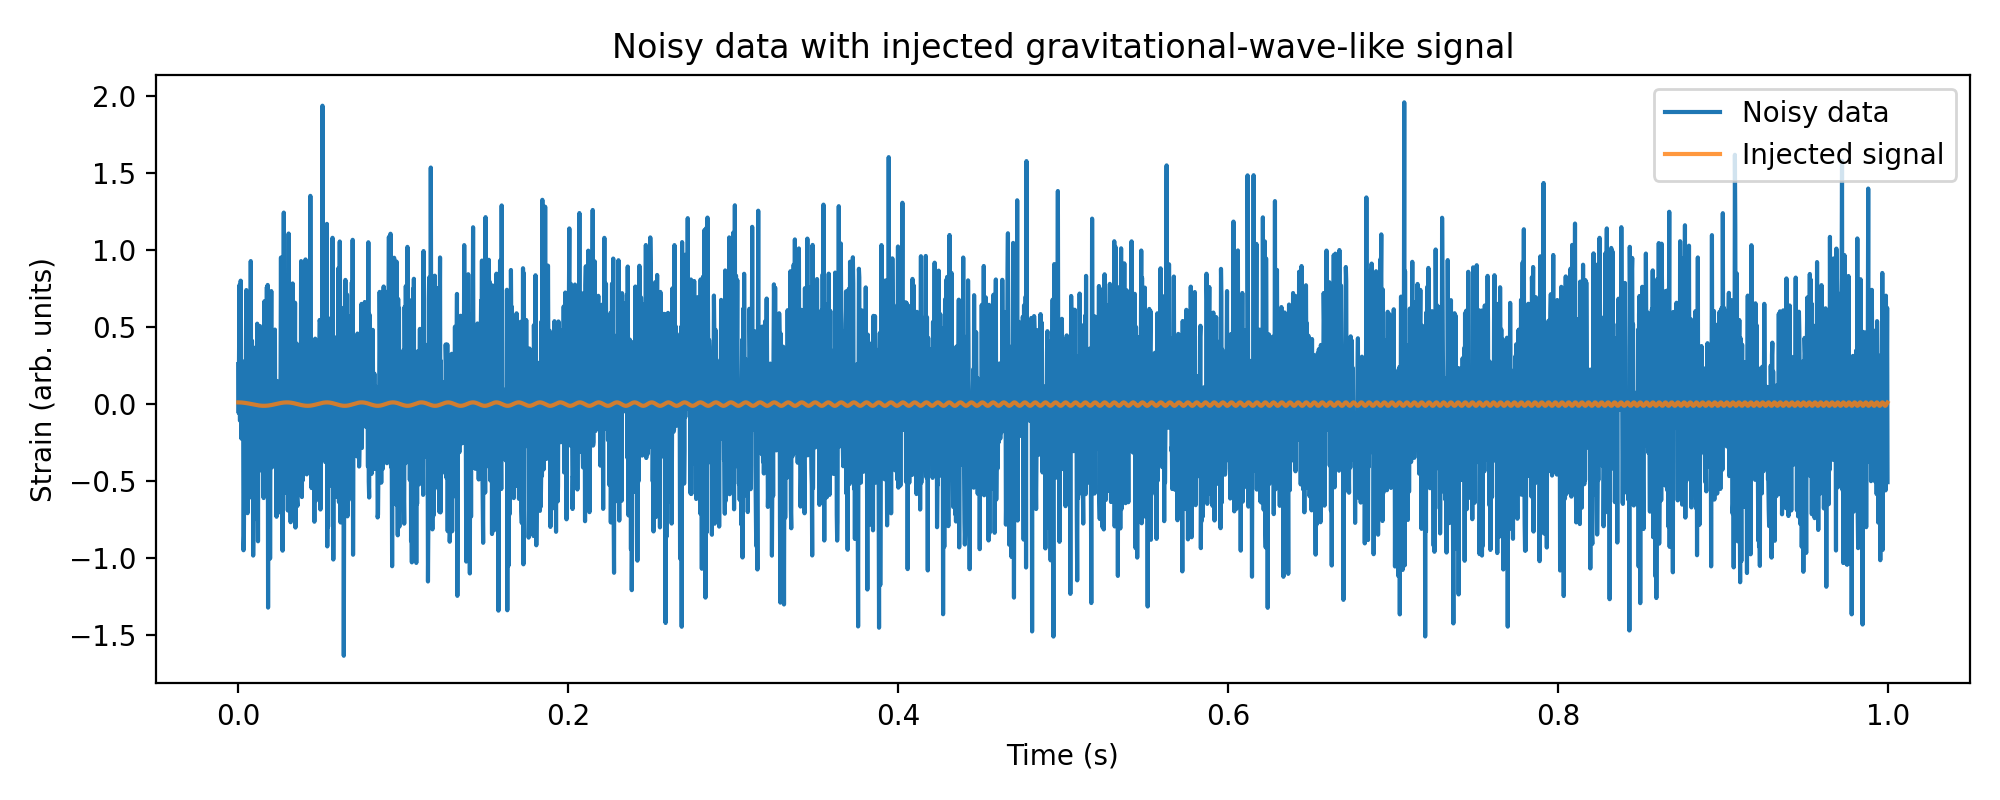
\includegraphics[width=0.95\linewidth]{fig1_timeseries.png}
\caption{Noisy data with injected chirp (unit-energy template scaled by an amplitude) overlaid.}
\end{figure}

\begin{figure}[h!]\centering
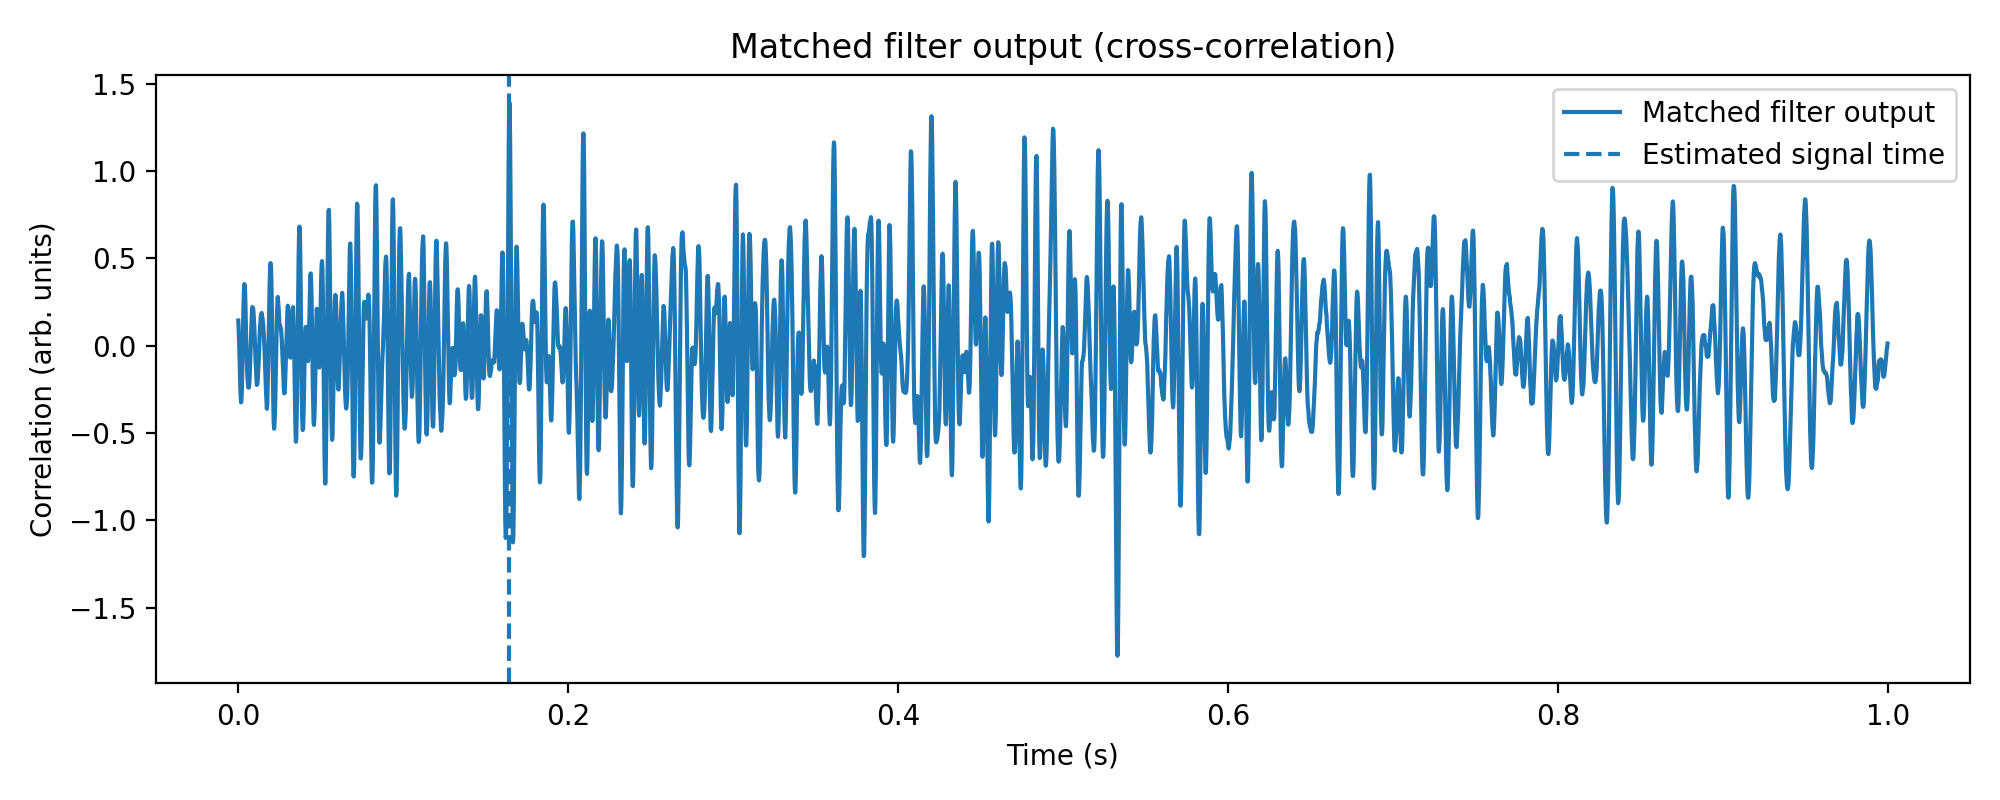
\includegraphics[width=0.95\linewidth]{fig2_correlation.png}
\caption{Matched-filter output (toy correlation) vs.\ time. The dashed line marks the peak (estimated arrival time).}
\end{figure}

\begin{figure}[h!]\centering
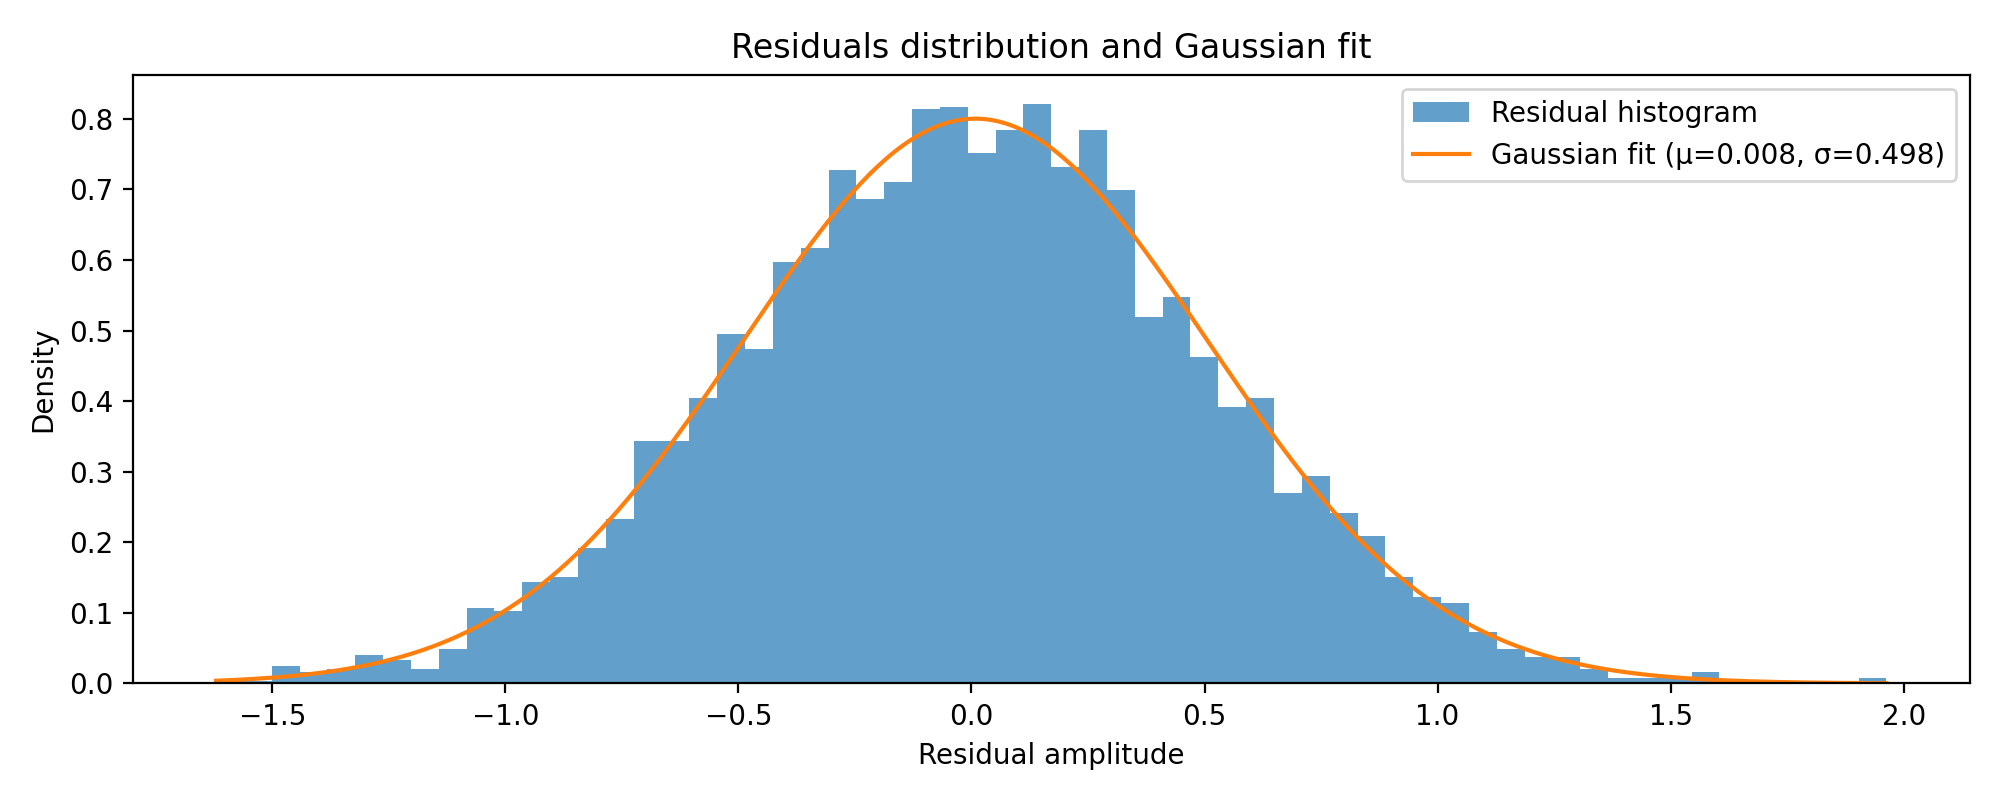
\includegraphics[width=0.95\linewidth]{fig3_residual_hist.png}
\caption{Residual histogram with Gaussian fit. This is the operational meaning of ``Gaussian'': a bell-shaped distribution with predictable tails.}
\end{figure}

\begin{figure}[h!]\centering
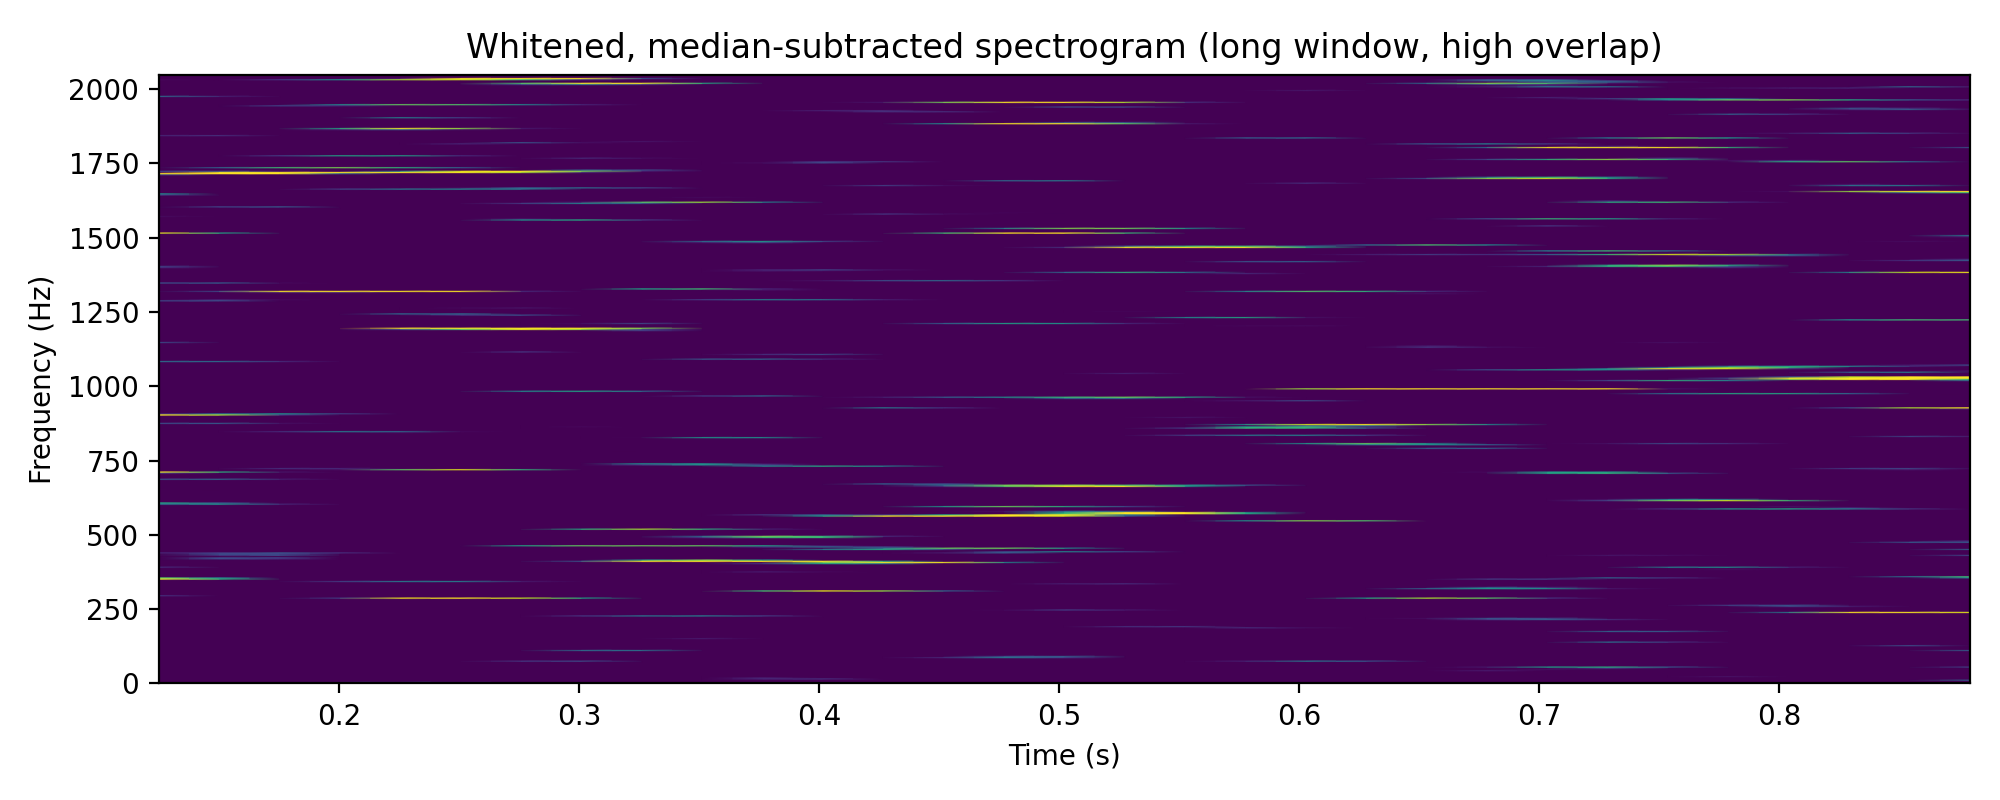
\includegraphics[width=0.95\linewidth]{fig4_spectrogram.png}
\caption{Whitened, median-subtracted spectrogram using a long Hann window with 90\% overlap; color limits clipped to the 95th--99.5th percentiles.}
\end{figure}

\appendix
\section*{Parameters}
\noindent Table~\ref{tab:params} lists the parameters used in the experiment.
\begin{table}[h!]\centering
\caption{Parameters of the toy experiment.}
\label{tab:params}
\begin{tabular}{ll}
\toprule
Parameter & Value \\
\midrule
Sampling rate & 4096 Hz \\
Duration & 1.00 s \\
Chirp start frequency & 30.0 Hz \\
Chirp end frequency & 300.0 Hz \\
Signal amplitude & 0.50 \\
Noise std. dev. & 0.50 \\
Estimated arrival time & 0.1643 s \\
Approx. SNR (toy) & 3.38 \\
Residual μ, σ & 0.008, 0.498 \\
\bottomrule
\end{tabular}

\end{table}

\end{document}
